\newpage
\section{Технологический раздел}
\subsection{Язык программирования}
	При разработке программного продукта был использован язык программирования C$\#$. \cite{c} В качестве среды разработки была использована Visual Studio 2015. \cite{VS2015} Данный выбор обусловлен прежде всего тем, что именно эти инструменты привлекаются для разработки ПО на предприятии. \\
	
	Такой язык программирования был выбран в качестве основного на предприятии по нескольким причинам:
	\begin{enumerate}
		\item [1)] большое количество готовых библиотек и шаблонов;
		\item [2)] исчерпывающая документация;
		\item [3)] низкий порог вхождения;
		\item [4)] поддержка ООП.
	\end{enumerate}

\subsection{Используемые классы}
	На рисунке \ref{fig16:image} представлена UML-диаграмма классов.
	
	\begin{figure}[ph!]
		\centering
		\begin{center}
			{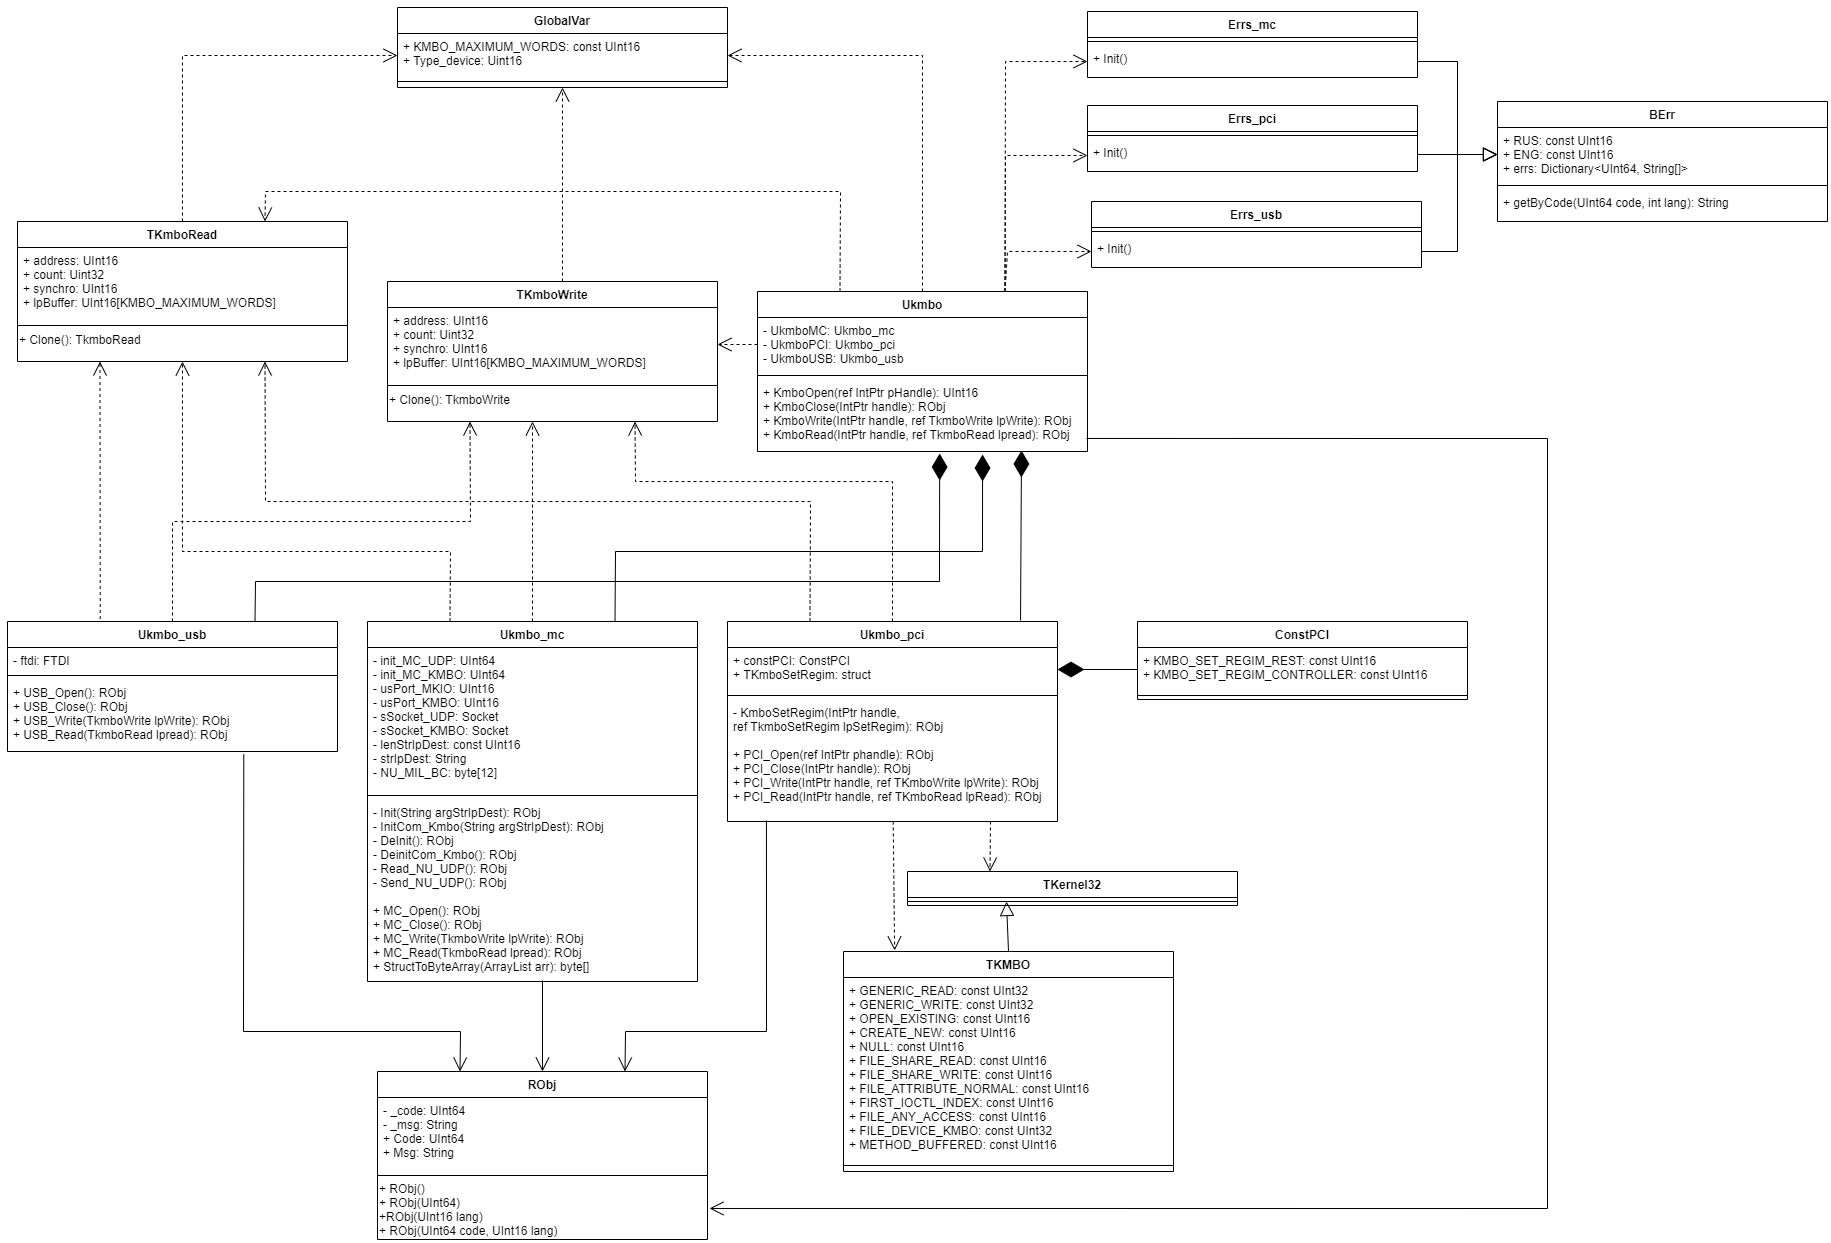
\includegraphics[scale=0.39, angle=90]{schemes/practice.png}}
			\caption{Используемые классы}
			\label{fig16:image}
		\end{center}
	\end{figure}

\newpage

\subsection{Используемые классы}
	\begin{enumerate}
		\item \textbf{Class GlobalVar}
		
		Класс глобальных переменных.
		
		\item \textbf{Class RObj}
		
		Класс возвращаемого значения, хранит код ошибки и соответствующую информацию, заполнение/изменение этого поля происходит одновременно с заданием/изменением поля кода ошибки. 
		
		\item \textbf{Class BErr}
		
		Базовый класс ошибки. Содержит метод getByCode(), который по коду ошибки находит соответствующую информацию о ней, сначала поиск осуществляется по заранее определённому словарю ошибок, в случае неудачи происходит обращение к WinAPI.
		
		\item \textbf{Class Errs$\_$mc}
		
		Класс ошибок, определённых для MC.
		
		\item \textbf{Class Errs$\_$usb}
		
		Класс ошибок, определённых для USB.
		
		\item \textbf{Class Errs$\_$pci}
		
		Класс ошибок, определённых для PCI.
		
		\item \textbf{Class TKMBO}
		
		Содержит необходимые для работы константы.
		
		\item \textbf{Class TKmboRead}
		
		Класс данных для чтения. \\
		Содержит поля адреса, количества записываемых слов, флаг, который определяет будет ли выводиться сигнал на осциллограф или нет и массив записанных слов.
		
		\item \textbf{Class TKmboWrite}
		
		Класс данных для записи. \\
		Содержит поля адреса, количества записываемых слов, флаг, который определяет будет ли выводиться сигнал на осциллограф или нет и массив записанных слов.
		
		\item \textbf{Class Ukmbo}
		
		Содержит основные методы взаимодействия с КМБО, такие как Open, Close, Read, Write.
		
		\item \textbf{Class Ukmbo$\_$mc}
		
		Содержит методы для взаимодействия с МС.
		
		\item \textbf{Class Ukmbo$\_$usb}
		
		Содержит методы для взаимодействия с USB.
		
		\item \textbf{Class ConstPCI}
		
		Класс констант, необходимых для взаимодействия с шиной PCI.
		
		\item \textbf{Class Ukmbo$\_$pci}
		
		Содержит методы для взаимодействия с PCI.
	\end{enumerate}

		Программная реализация классов представлена в приложениях А-Д.
		
	\subsection{Вывод}
	В этом разделе обосновывается выбор языка программирования и среды разработки, рассмотрена UML-диаграмма основных классов.


